\documentclass[main.tex]{subfiles}
\begin{document}

\begin{figure}[h]
\centering
\begin{minipage}{.45\textwidth}
	\centering
	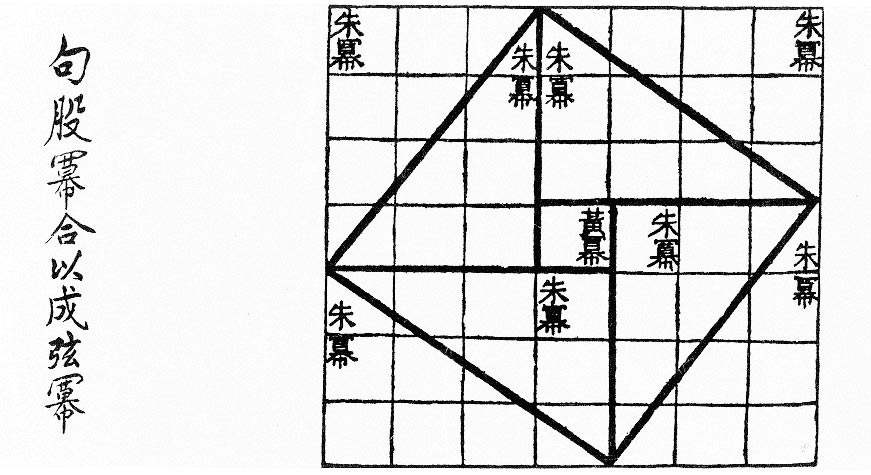
\includegraphics[width=0.8\textwidth]{jpg/gougu.jpg}
	%	\label{fig:1.5.2}
\end{minipage}
\begin{minipage}{.45\textwidth}
	\centering
	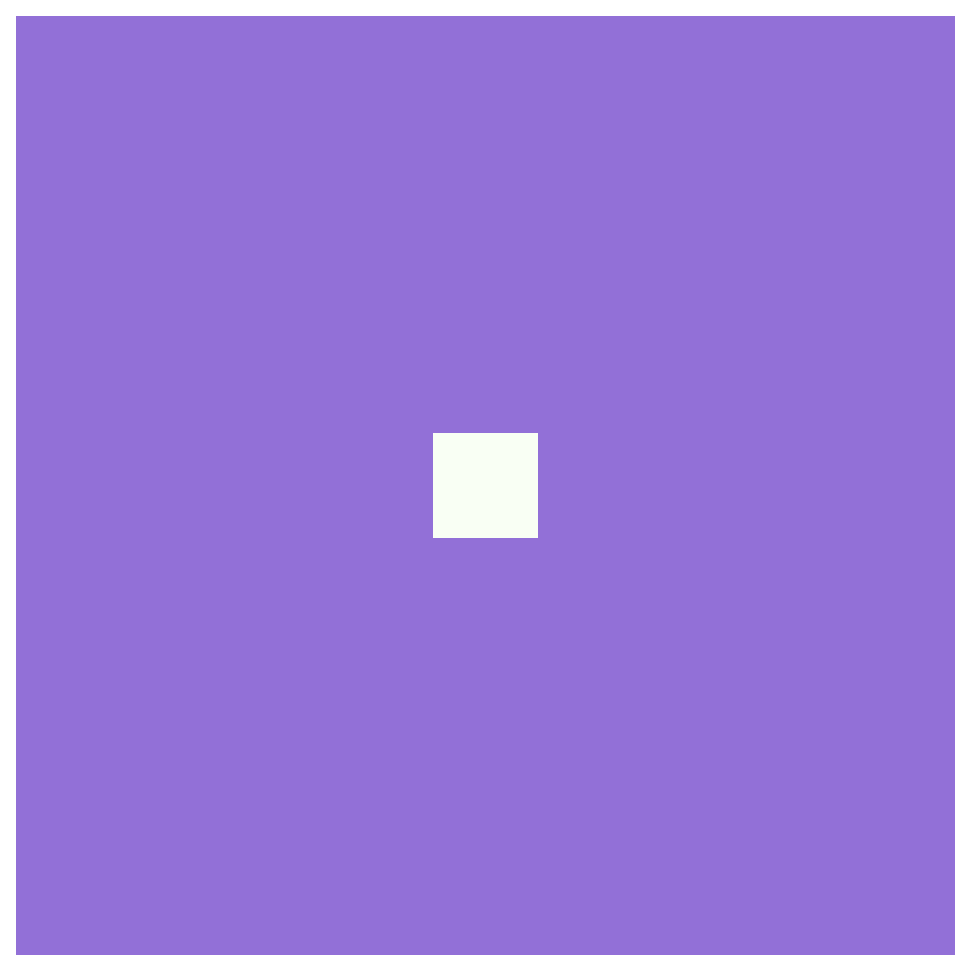
\includegraphics[width=0.44\textwidth]{eps/gougu.eps}
%    \label{fig:chap1.5.1}
\end{minipage}
\caption{勾股定理}
 \label{fig:1.5.1}
\end{figure}	

{《周髀算经》勾股定理图}

勾股定理 - 北京2002年国际数学家大会会标中的图案
\begin{figure}[h]
	\centering
	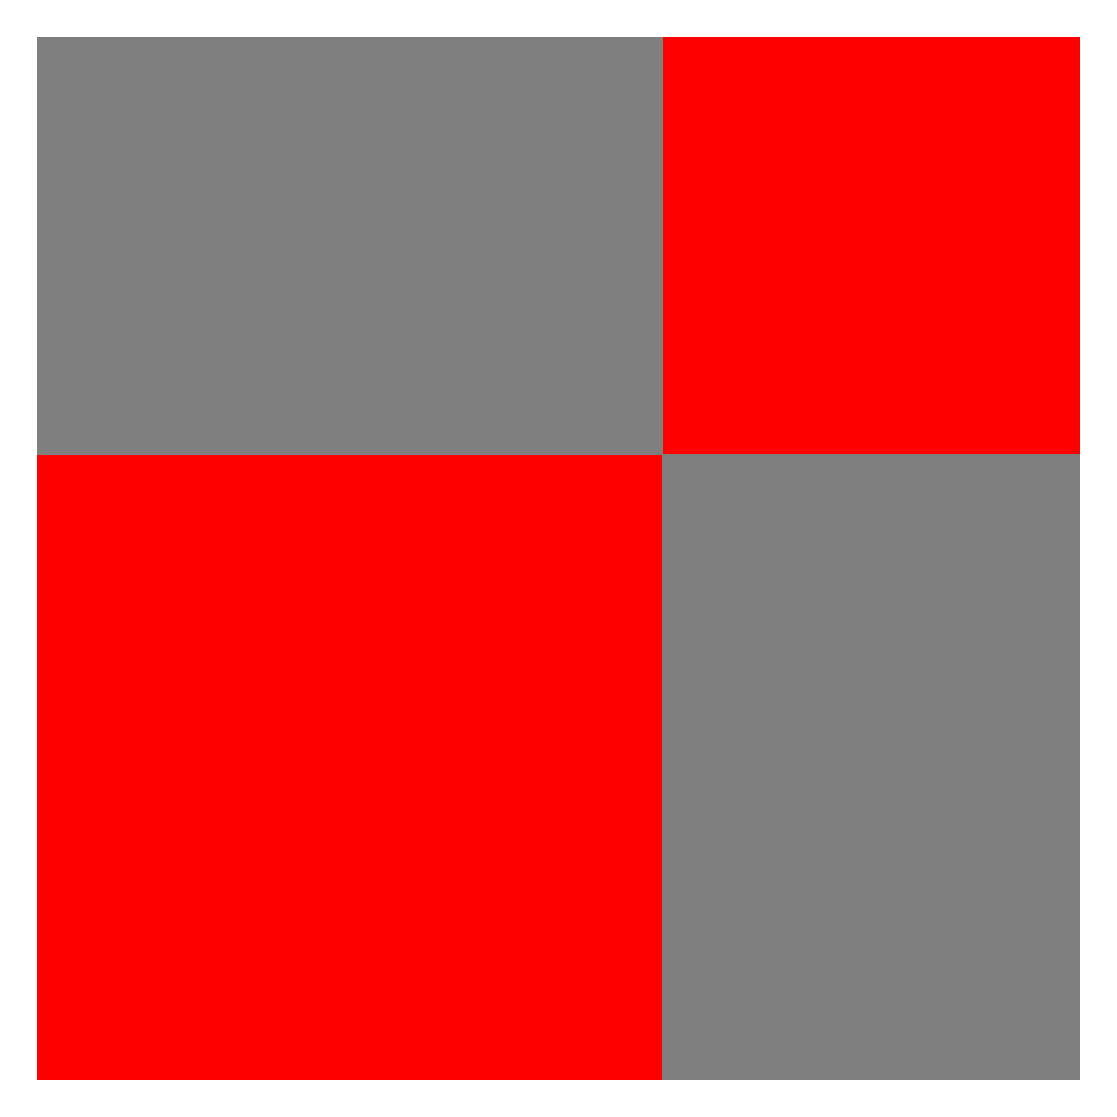
\includegraphics[width=0.5\textwidth]{eps/ps.1.1.eps}
	\caption{$(a+b)^2 = a^2 + 2ab + b^2$}
	\label{fig:chap1.5.3}
\end{figure}	



\end{document} 
